\documentclass{beamer}
\usepackage{amsmath,amssymb,amsfonts,latexsym,stmaryrd}
\usepackage[latin1]{inputenc}
\usepackage[T1]{fontenc}
% Conversi�n eps to pdf, requiere habilitar shell-escape.
% Texlive 2010 o superior No lo necesita
%\usepackage{epstopdf}
%\DeclareGraphicsExtensions{.pdf,.png,.jpg}
\usefonttheme{professionalfonts} % fuentes de LaTeX
\usetheme{Warsaw} % Tema escogido en este ejemplo
\setbeamercovered{transparent} % Velos
\newtheorem{teo}{Teorema}
\newtheorem{ejemplo}{Ejemplo}
\newtheorem{defi}{Definici�n}
\newtheorem{coro}{Corolario}
\newtheorem{prueba}{Prueba}
\usepackage[ruled,vlined,lined,linesnumbered,algosection,spanish]{algorithm2e}
\usepackage{multimedia}
\begin{document}
\parbox{3cm}{
\href{http://www.tec-digital.itcr.ac.cr/revistamatematica/cursos-linea/
3D-Web/exersolido21.html}{
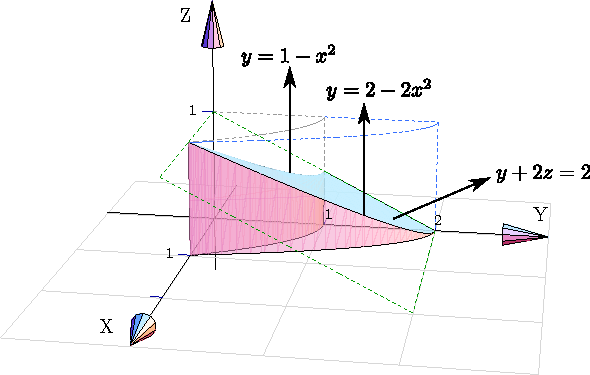
\includegraphics[width =3cm]{images/exersolido21}}
}\parbox{12cm}{S�lido $Q_{14}$ limitado por las
superficies $y=2-2x^2;$ $y=1-x^2;\;\;y+2z=2;\;\;x=0$ y $z=0;$ en el
I octante.}\\
\end{document}